%% ----------------------------------------------------------------
%% Thesis.tex -- MAIN FILE (the one that you compile with LaTeX)
%% ---------------------------------------------------------------- 

% Set up the document
\documentclass[a4paper, 11pt, oneside]{Thesis}  % Use the "Thesis" style, based on the ECS Thesis style by Steve Gunn
\graphicspath{{./Figures/}}  % Location of the graphics files (set up for graphics to be in PDF format)

% Include any extra LaTeX packages required
\usepackage[ ]{biblatex}
\addbibresource{library.bib}
\addbibresource{inhand.bib}
\addbibresource{webs.bib}
\usepackage{verbatim}  % Needed for the "comment" environment to make LaTeX comments
\usepackage{vector}  % Allows "\bvec{}" and "\buvec{}" for "blackboard" style bold vectors in maths
\hypersetup{urlcolor=blue, colorlinks=true}  % Colours hyperlinks in blue, but this can be distracting if there are many links.
\usepackage{multirow}
\usepackage{makecell}
\usepackage[capitalise]{cleveref}
\usepackage{listings}

\begin{document}
%% ----- Cover ----------------------------------------------------
  \frontmatter      % Begin Roman style (i, ii, iii, iv...) page numbering

  % Set up the Title Page
  \title {Autonomous Navigation Behaviors for an Aerial Robotics Software Framework}
  \authors {
    \texorpdfstring{
      Guillermo Echegoyen Blanco
    }
    {Guillermo Echegoyen Blanco}
  }
  \addresses {
    \groupname\\\deptname\\\univname
  }  % Do not change this here, instead these must be set in the "Thesis.cls" file, please look through it instead
  \date {\the\year}
  \subject {}
  \keywords {}

  \maketitle
%% ----------------------------------------------------------------
%% ----- Page Setup -----------------------------------------------
  \setstretch{1.3}  % It is better to have smaller font and larger line spacing than the other way round

  % Define the page headers using the FancyHdr package and set up for one-sided printing
  \fancyhead{}  % Clears all page headers and footers
  \rhead{\thepage}  % Sets the right side header to show the page number
  \lhead{}  % Clears the left side page header

  \pagestyle{fancy}  % Finally, use the "fancy" page style to implement the FancyHdr headers
%% ----------------------------------------------------------------
%% ----- Declaration Page -----------------------------------------
  % Declaration Page required for the Thesis, your institution may give you a different text to place here
  % \Declaration{

  %   \addtocontents{toc}{\vspace{1em}}  % Add a gap in the Contents, for aesthetics

  %   I, AUTHOR NAME, declare that this thesis titled, `THESIS TITLE' and the work presented in it are my own. I confirm that:

  %   \begin{itemize} 
  %     \item[\tiny{$\blacksquare$}] This work was done wholly or mainly while in candidature for a research degree at this University.
  %      
  %     \item[\tiny{$\blacksquare$}] Where any part of this thesis has previously been submitted for a degree or any other qualification at this University or any other institution, this has been clearly stated.
  %      
  %     \item[\tiny{$\blacksquare$}] Where I have consulted the published work of others, this is always clearly attributed.
  %      
  %     \item[\tiny{$\blacksquare$}] Where I have quoted from the work of others, the source is always given. With the exception of such quotations, this thesis is entirely my own work.
  %      
  %     \item[\tiny{$\blacksquare$}] I have acknowledged all main sources of help.
  %      
  %     \item[\tiny{$\blacksquare$}] Where the thesis is based on work done by myself jointly with others, I have made clear exactly what was done by others and what I have contributed myself.
  %     \\
  %   \end{itemize}
  %  
  %    
  %   Signed:\\
  %   \rule[1em]{25em}{0.5pt}  % This prints a line for the signature
  %    
  %   Date:\\
  %   \rule[1em]{25em}{0.5pt}  % This prints a line to write the date
  % }
  % \clearpage  % Declaration ended, now start a new page
%% ----------------------------------------------------------------
%% ----- Funny Quote ----------------------------------------------
  % The "Funny Quote Page"
  \pagestyle{empty}  % No headers or footers for the following pages

  \null\vfill
  % Now comes the "Funny Quote", written in italics
  \textit{``The Situation is Hopeless But Not Serious.''}

  \begin{flushright}
    Paul Watzlawick
  \end{flushright}

  \vfill\vfill\vfill\vfill\vfill\vfill\null
  \clearpage  % Funny Quote page ended, start a new page
%% ----------------------------------------------------------------
%% ----- Abstract Page --------------------------------------------
  % The Abstract Page
  \addtotoc{Abstract}  % Add the "Abstract" page entry to the Contents
  \abstract{
    \addtocontents{toc}{\vspace{1em}}  % Add a gap in the Contents, for aesthetics
    In the present work we propose an autonomous navigation system for aerial robotics. Based on the state of the art literature for localization, mapping and planning and the use of the Aerostack software platform we implement a system capable of executing navigation tasks in an autonomous way.

    We validate our findings and test our software through the implementation of a mission based on an industrial necessity and run it both in real flight and simulation. The main findings and results are reported and discussed along with the promising future we find for this system.
  }
  \clearpage  % Abstract ended, start a new page
%% ----------------------------------------------------------------
%% ----- Acknowledgements page ------------------------------------
  \setstretch{1.3}  % Reset the line-spacing to 1.3 for body text (if it has changed)
  % The Acknowledgements page, for thanking everyone
  \acknowledgements{
    \addtocontents{toc}{\vspace{1em}}  % Add a gap in the Contents, for aesthetics
    To my project advisor for his supervision, long chats and help with the figures.

    To the inhabitants of the \textit{great flat}, both the regular and the constants. Without their endless patience and support this would have never been possible. They have encouraged me to work harder and cheer up on the worst moments.

    To my father, for his lifelong lessons on perseverance and tolerance.
  }
  \clearpage  % End of the Acknowledgements
%% ----------------------------------------------------------------
%% ----------------------------------------------------------------
%% ----- Contents, List of Figures, List of Tables ----------------
  \pagestyle{fancy}  %The page style headers have been "empty" all this time, now use the "fancy" headers as defined before to bring them back
  
  \lhead{\emph{Contents}}  % Set the left side page header to "Contents"
  \tableofcontents  % Write out the Table of Contents
  
  \lhead{\emph{List of Figures}}  % Set the left side page header to "List if Figures"
  \listoffigures  % Write out the List of Figures

  \lhead{\emph{List of Tables}}  % Set the left side page header to "List of Tables"
  \listoftables  % Write out the List of Tables
  \setstretch{1.5}  % Set the line spacing to 1.5, this makes the following tables easier to read
  \clearpage  % Start a new page
%% ----------------------------------------------------------------
%% ----- Abbreviations, Physical Constants, Symbols ---------------
  \begin{comment}
  \lhead{\emph{Abbreviations}}  % Set the left side page header to "Abbreviations"
  \listofsymbols{ll}  % Include a list of Abbreviations (a table of two columns)
  {
    % \textbf{Acronym} & \textbf{W}hat (it) \textbf{S}tands \textbf{F}or \\
    % \textbf{LAH} & \textbf{L}ist \textbf{A}bbreviations \textbf{H}ere \\
  }
  \clearpage  % Start a new page

  \lhead{\emph{Physical Constants}}  % Set the left side page header to "Physical Constants"
  \listofconstants{lrcl}  % Include a list of Physical Constants (a four column table)
  {
    % Constant Name & Symbol & = & Constant Value (with units) \\
    % Speed of Light & $c$ & $=$ & $2.997\ 924\ 58\times10^{8}\ \mbox{ms}^{-\mbox{s}}$ (exact)\\
  }
  \clearpage  %Start a new page

  \lhead{\emph{Symbols}}  % Set the left side page header to "Symbols"
  \listofnomenclature{lll}  % Include a list of Symbols (a three column table)
  {
    % symbol & name & unit \\
    % $a$ & distance & m \\
    % & & \\ % Gap to separate the Roman symbols from the Greek
    % $\omega$ & angular frequency & rads$^{-1}$ \\
  }
  \end{comment}
%% ----------------------------------------------------------------
% End of the pre-able, contents and lists of things
%% ----- Dedication Page ------------------------------------------
  % Begin the Dedication page
 %  \setstretch{1.3}  % Return the line spacing back to 1.3

 %  \pagestyle{empty}  % Page style needs to be empty for this page
 %  \dedicatory{For/Dedicated to/To my\ldots}

 %  \addtocontents{toc}{\vspace{2em}}  % Add a gap in the Contents, for aesthetics
%% ----------------------------------------------------------------
%% ----- Main Document --------------------------------------------
  \mainmatter   % Begin normal, numeric (1,2,3...) page numbering
  \pagestyle{fancy}  % Return the page headers back to the "fancy" style

  \renewcommand{\chaptermark}[1]{\markboth{#1}{}} % Make the chapter mark without the "Chapter X" stuff
  \lhead{\emph{\leftmark}}  % Set the left side page header accordingly

  \chapter{Introduction}

  In the following work an integration of a navigation system onto the Aerostack platform is presented.

  \section{Context}

    Aerostack is a framework for aerial robots, aimed at giving flight autonomy to some extent. It features a modular approach for the construction of behaviors that can be used to develop complex flights and automatic handling for certain situations such battery level or hardware conditions. It is the frame for the following work, which adds more autonomy through the integration of a octomap-based navigation system and a global planner. This provides a novel localization technique for the framework.

  \section{Motivation}

    So far, there exists only one simple geometry planner and an Aruco-based localization technique. In indoor environments, this system compels the need for environment preparation, the Arucos must be placed beforehand in well known localizations that must be hardcoded in the robot map. In this sense, there exists a need for a more robust, preparation-free localization system and accompanying planner. This work provides such an improvement with the introduction of a octomap-based navigation system and a global planner.

  \section{General Objective}

    This work aims at adding a novel navigation system to the Aerostack framework.


  \section{Specific Objectives}

    This section enumerates a comprehensive list of objectives.

    \begin{enumerate}
      \item Enrich the current navigation and localization systems.
      \item Test and validate the new navigation and localization systems through simulated environments.
    \end{enumerate}

    To achieve the first objective, the following additions to the framework are proposed:

    \begin{itemize}
      \item Add a robust planner based on a new navigation technique.
      \item Add a robust navigation technique through the use of octomaps.
      \item Add a robust localization technique based on octomaps.
      \item Add octomaps construction support through lidar.
    \end{itemize}

  \section{Overview}

    \textbf{[ToDo := Review when everything is finished]}

    This dissertation is organized as follows: ...

 % Introduction
  \chapter{Problem Description}

  In the present chapter the problem is presented, along with an introduction to the previous work. It is structured as follows: Section \ref{ch_2:sect:1} presents the context of the problem and the requirements a replacement should have. Section \ref{ch_2:sect:2} describes deeply the improvements presented and the decisions taken to end in Section \ref{ch_2:sect:3} with the description of the previous system.

  \section{Requirements} \label{ch_2:sect:1}

    As of the second version of Aerostack, the only localization technique available is based on the recognition of a special type of marker called Aruco, first used for augmented reality applications. It is a fast and reliable technique to estimate the pose of the camera capturing the image. Altough this system works fine for many applications, it imposes the need of preparing the environment, placing this markers in a very precise way and annotating it's exact position before the experiments. While this might not be a problem in an augmented reality like scenario, when it comes to live localization in unknown environment it becomes useless. Hence, a new system for localization is required.

    Along with the aforementioned localization technique comes the navigator which coordinates with a 2D geometric planner to accomplish the mission at hand. As the localization technique is to be changed, leading to a new way to perceive the environment, a new navigator and planner will be necessary. 

  \section{Details of the New Features} \label{ch_2:sect:2}

    A lidar is going to be used as the main source for localization. The module in charge of this part is already present in the Aerostack framework, but it is not being used. Based on lidar input an octomap is built. This octomap is then used by the navigator, along with the planner instructions to build a motion plan to execute.

    The lidar + octomap functionality is provided by a module called hector\_slam, developed at the Darmstadt University \cite{hector_slam}. Taking the lidar's cloud of points it is able to reconstruct an octomap and then localize inside it (SLAM). The output of this module can be used to create a plan avoiding obstacles to reach a target point.

    [ ToDo := Review, NavStack \& Global Planner ]

  \section{Previous Work} \label{ch_2:sect:3}

    By now, there is a process responsible for doing recognition of Aruco markers, it is connected to the robot camera and fetches data every $n$ milliseconds, where $n$ is a user defined constant. When an aruco is recognized, the pose of the robot can be estimated. Knowing the exact position of the marker enables the process to estimate the absolute position of the robot, leading to a high precision coordinates localization. While this approach has many advantages, it fails when the environment is not prepared beforehand.

    To create a plan, a target position and the used Aruco markers are specified, then the motion planner creates a 2D plan to follow, using the Arucos to localize in the process.

    \begin{comment}
      \begin{itemize}
      \end{itemize}
    \end{comment}

 
  \chapter{State of the Art}

  This chapter will review the classic methods used for localization and mapping, which is the core for any navigation technique, it starts describing the problems that arise both in localization and mapping. Continue with some of the most prolific solutions found to these problems to finish exposing the techniques and algorithms used by the Aerostack framework.

  Localization is referred to all the techniques used to find the position in coordinates of an agent or object inside the world, relative to a reference frame. As far as it's absolute coordinates are known, anything can be used as reference frame, it is used as the coordinates system's centre. In an outdoors environment, the Earth could be the reference frame and the robot's coordinates can be acquired with satellite systems, giving an absolute point inside the three dimensional space. It is desirable for these coordinates to be in a format that a computer can handle efficiently, tipically as two or three floating point numbers (although integer numbers are used sometimes too), depending on the number of dimensions used to represent the space. To save computational effort, the z axis (height) could be unused in a wheeled robot.

  Moving a robot avoiding possible obstacles through the space is tricky in itself, obstacles must be detected and handled correctly, moving objects can appear in the way, and so on. This alone does not provide any intelligence nor it helps planning, to aid in planning and moving smartly in the space, a map can be constructed while the localization is happening. The term mapping covers all the algorithms used to construct a map combining the data acquired from the many input sources a robot can have. Mapping opens the door for smart planning, along with many more advantages. A classic example is finding cycles in planned paths.

  \clearpage

  \section{Localization}

    Localization techniques are divided into two groups: Outdoor and indoor techniques. The distinction comes from the fact that satellite systems signals cannot go through walls. This fact has led to a whole new set of technologies and techniques that are able to localize in environments without an absolute reference of the world.

    This section is organized as follows: First outdoor localization will be analyzed, with a brief review of it's core components, then various indoor localization techniques will be exposed, focusing on lidar based techniques.

    \subsection{Outdoor localization} \label{ch_3:sect:localization:outdoor}

      By now, the most robust, reliable solution for outdoor localization is based on combining different sources of data. The mobile platform has drawn great attention over the past few years, pushing some of the largest companies in a shared effort to improve localization services while minimizing the impact over the battery's performance.

      Satellite systems localization in mobile applications have certain drawbacks: The most obvious one is that acquiring and processing the signal wastes power, but also that in the case of civilian systems (such as GPS) the localization has a precision of 10 meters for security reasons. Figure \ref{ch_3:fig:trilateration} shows the localization dissambiguation through the trilateration technique with three satellite.

      To aid both problems two new localization techniques were implemented:
      \begin{enumerate}
        \item GSM Localization. As every GSM antenna has a well known location stored in a database, one can localize trilaterating the near GSM antennas. Obviosly, this method is subject to GSM signal coverage.
        \item WiFi Localization. This powerful method can serve both as an indoor and outdoor localization technique (see sect. \ref{ch_3:sect:localization:indoor}). When a smarphone detects a WiFi hotspot, it sends it's BSSID along with the GPS coordinates if available to a centralized server. As this database grows the localization precision improves and every user can take advantage from it. This is scpecially useful in urban areas where stallite signal is poor or intermitent and improves as more and more users log information.
      \end{enumerate}

      The best localization services can be provided with the conjunction of these three main techniques, which can be easily merged with an \textit{Extended Kalman Filter}.

      \begin{figure}
        \centering
        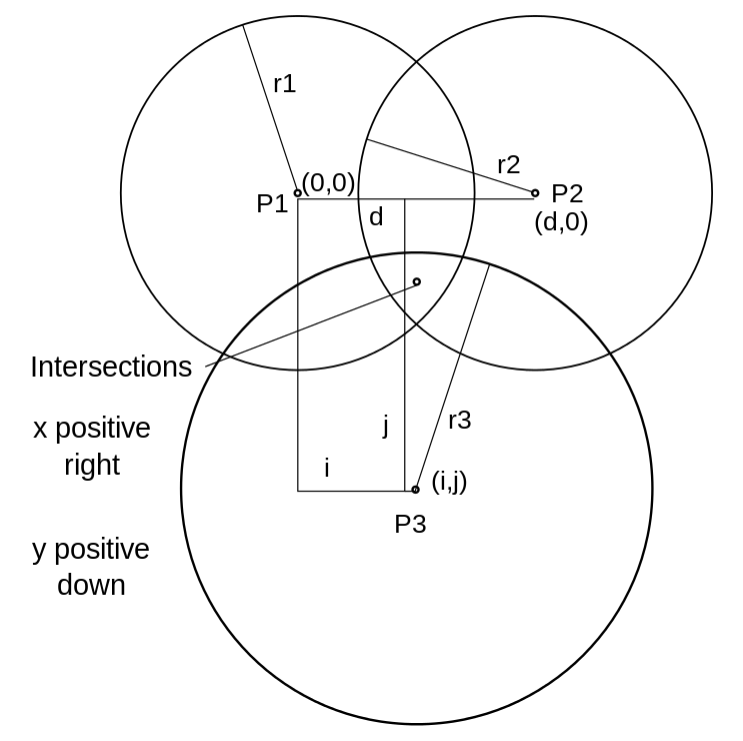
\includegraphics[width=0.6\textwidth]{./Figures/trilateration.png}
        \caption{The area enclosed by the three intersections ca be used to localize univocally. The three simple intersections formed by pairs of circumferences are always outside of the Earth. As more satellites are included, precision increases. Taken from \cite{wikipedia_trilateration_web}.}
        \label{ch_3:fig:trilateration}
      \end{figure}

      Although these techniques are widely used they are limited to mobile platforms, which are restricted both in sensorization and in processing capabilities. For robotic applications more sophisticated sensors are used, this includes depth cameras and lidars for the most part. Again, all the sensors output is merged to get the best estimates.

      In robotics, it is usual that the localization we are interested in is relative instead of absolute. This is done to aid in locating near objects in the space relative to the robot but also to construct a map, the process of localization and mapping simultaneously is called \textit{SLAM - Simultaneous Localization And Mapping} (see sect. \ref{ch_3:sect:localization:slam}).

    \subsection{Indoor localization} \label{ch_3:sect:localization:indoor}

      To localize in indoor environments many strategies can be followed, the general trend is to place different markers (active or passive) beforehand in well known locations. This markers are then recognized by the localizing device to know it's location. This \textit{recognizable markers} can be anything, a Bluetooth beacon, a WiFi hotspot, etc.

      Bluetooth beacons are specially crafted for this purpose as they can provide much more information. It has been extensively used in congresses and hotels to provide hosts with more information beyond localization, as services and timetables based on location. 

      In the case of WiFi hotspots localization is usually done by analyzing the signal strength and incoming angle. This method only works when the hotspots' location is known beforehand and is very prone to errors because the device must remain static in a certain angle.

      From the computer vision perspective, visual markers can be placed too and processed by the device localizing and again, this requires preparation beforehand. One example of this setup are the well known \cite{romeroramirez201838}.

      In many robotic applications like swarm robotics there is a necessity to track each member of the swarm in a closed, contained environment, for this purpose an OptiTrack system \cite{optitrack_web} can be used, it is a highly precise camera set that can track various markers (marked swarm members) and serve it's location through the network in real time. This setup is specially useful to monitor the swarm, enabling each member to access it's location.

    \subsection{SLAM} \label{ch_3:sect:localization:slam}

      SLAM is the process of mapping and, at the same time localizing inside that map. This is particularly useful in environments that are not prepared like the ones exposed previously, enabling the robot to work on an unknown place without getting lost nor entering cyclic paths. SLAM techniques are crucial in any robot with some degree of autonomy, it makes the navigation possible. 

      There are three main variants here, the ones based on Extended Kalman Filters, the probabilistic ones and the ones based on Graph Optimization.

    \subsubsection{Extended Kalman Filters SLAM} \label{ch_3:sect:localization:ekf}

      Extended Kalman Filters (EKF) SLAM is the earliest technique developed for SLAM. EKF is a general technique to find the best estimate for the measuring variable based on the mean and covariance. In this case the inputs are the odometry used to estimate the robot position, features of the environment that anchor the odometry measures and the robot motor system sensors (wheel decoders, etc) to estimate the change on the position. Then the objective is to find the best estimate for the current robot's position.

      \begin{figure}[!t]
        \centering
        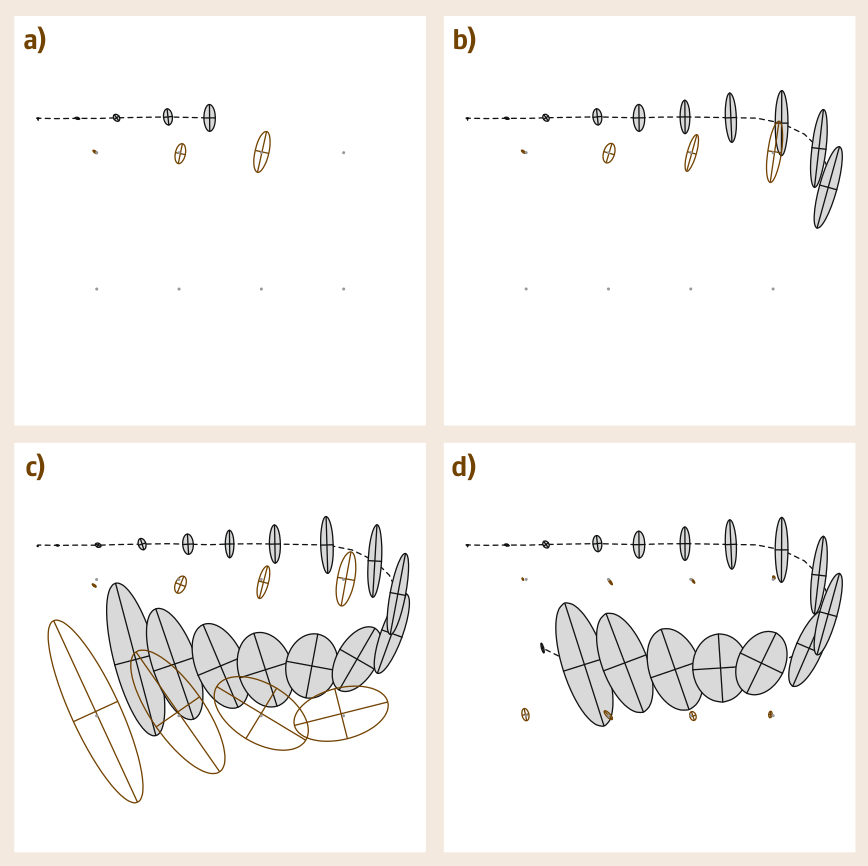
\includegraphics[width=0.8\textwidth]{./Figures/slam_ekf_model.png}
        \caption{EKF applied to the SLAM problem. Dotted line: robot's path. Shaded ellipses: position estimates. Small dots: Unkown location landmarks. White ellipses: Landmarks' position estimates. In (d) the robot senses the first landmark, anchoring the rest of the estimates, reducing uncertainty. Taken from \cite{inbookhandbook}}
        \label{ch_3:fig:ekf_slam}
      \end{figure}

      At the start of the process, the system's ($0$, $0$) coordinate is established where the robot is, this is the most confident measure about the robot position. As the robot navigates the environment, succesive measures are taken and paired with the known landmarks, when a previously seen landmark is witnessed again, the position estimate is corrected with the covariance matrix, and the error correction is propagated along the previous estimates. In this way a long as the robot is navigating an sensing the landmarks, the position estimate improves. Figure \ref{ch_3:fig:ekf_slam} shows the full process, in (a) the process is started, there is a lot of uncertainty, as process continues (a-c) the uncertainty increases, until the first landmark is sensed again (c), reducing the uncertainty on the current position's estimate and the subsequent estimates.

      More formally, the EKF algorithm represents the robot estimate by a multivariate Gaussian (\ref{ch_3:eq:ekf_representation})
      
      \begin{equation} \label{ch_3:eq:ekf_representation}
        p(x_{t}, m | Z_{t}, U_{t}) = N(\mu_{t}, \Sigma_{t})
      \end{equation}

      Where $\mu_{t}$ contains the robot's best estimate of its current location $x_{t}$ and the locations of all the landmarks, its size is $3 + 2N$, 3 points for the robot location and 2 for each of the $N$ landmarks. The matrix $\Sigma_{t}$ is the covariance of the expected error in the guess $\mu_{t}$ assessed by the robot, a square, dense matrix of $(3 + 2N) \times (3 + 2N)$.

      Although this technique works well on small maps, it renders unusable for large maps, this happens because the covariance matrix $\Sigma_{t}$ used to correlate the position estimates grows cuadratically with the measures, making the memory footprint wildly large and the overall processing time very high. Some researchers have proposed an improvement over the EKF SLAM algorithm through submap decomposition \cite{Guivant2001, Leonard2000}.

    \subsubsection{Particle Filters}

      Particle Filters are a probabilistic approach to position estimation, usually called Fast SLAM \cite{Montemerlo2002}. It uses various \textit{particles} that represent the posterior probability of the true distribution of maps and possible paths. To do so it stands over a method called Rao-Blackwellization, that aids in dimensioning the number of particles needed to represent the map. Also, as conditional indepence is assumed between the observed landmarks, every landmark can be represented as $N$ small Gaussians, which is linear, instead of exponential on the number of landmarks.

      At any point a set of $K$ particles is retained, where each particle has the form exposed in equation \ref{ch_3:eq:particle_form}.

      \begin{equation} \label{ch_3:eq:particle_form}
        X_{t}^{[k]}, \mu_{t,1}^{[k]}, \cdots, \mu_{t,N}^{[k]}, \Sigma_{t,1}^{[k]}, \cdots, \Sigma_{t,N}^{[k]}
      \end{equation}

      Where $k$ is the index of the path sample and $n$ the number of the landmark. This implies that every particle contains a sample path $X_{t}^{[k]}$ and a set of $N$ Gaussians $\approx (\mu_{t,n}^{[k]}, \Sigma_{t,n}^{[k]})$, one for each landmark.

      When a new odometry measure is received, it is combined with the previous knowledge through probabilistic sampling. A new location is generated for each particle, following a distribution based on the robot motion model and the previous measure of that particle ($x_{t-1}^{[k]}$). More specifically:

      \begin{equation} \label{ch_3:eq:particle_update}
        x_{t}^{[k]} \approach p(x_{t} | x_{t-1}^{[k]}, u_{t})
      \end{equation}

      Then, when a new measure $z_{t}$ is received, each particle's importance is weighted, assigning how important is that particle to that measure, this is the probability of that measure based on the particle's knowledge, defined in equaton \ref{ch_3:eq:particle_importance}. Let $n$ be the observed landmark's index:

      \begin{equation} \label{ch_3:eq:particle_importance}
        w_{t}^{[k]} = N(z_{t} | x_{t}^{[k]}, \mu_{t,n}^{[k]}, \Sigma_{t,n}^{[k]})
      \end{equation}

      After equation \ref{ch_3:eq:particle_importance} is applied for each particle, all the weights are normalized to sum up to 1, then a set new particles is drawn with replacement, where the probability of being picked is each particle weigth. Intuitively, this means that only the particles that fit the most with the current measures survive for next rounds. The final step of FastSLAM updates the mean $\mu_{t}^{[k]}$ and covariance $\Sigma_{t,n}^{[k]}$ based on the new measure $z_{t}$, which is similar to the EKF updates, but with much smaller filters.

      Although this method is easy to implement, fast enough for real time applications with not very high demanding software and yields good results on small to medium maps, it suffers from the fact that lots of particles are needed to represent big maps, specially with multiple nested loops. Therefore, many improvements have been proposed, \cite{Grisetti2007} for example uses ocucupancy grids instead of Gaussians.

    \subsubsection{Graph Optimization SLAM}

      The Graph Optimization SLAM techniques try to optimize a graphical model representing the landmarks and robot locations. In this representation, each location is viewed as a node in the graph, and the edge (called soft constraint) between two consecutive nodes is the captured odometry. The key intuition behind these methods is that at the end, the graph is sparse, because, each node will have just a few connections to other nodes. Also, at worst, the number of entries in the graph is linear in the time elapsed and in the number of nodes.

      This is the most widely used approach because sparse linear optimization is in a very advanced stage, allowing for scalable, yet efficient implementations of the algorithm.

    \subsubsection{Lidar SLAM}

      Lidar is a well established laser range sensor that can be used for depth estimation. By doing fast sweeps in 360 degrees it can compose a depth map which can be used for SLAM.

      Hector SLAM \cite{hector_slam} is a technique developed in the Darmstadt University. It uses a lidar sensor to do a fast SLAM by matching rays along sweeps.

      Along this work, the \textit{hector\_slam} ROS module will be integrated into the Aerostack framework, providing a robust SLAM technique ready to use for the drones equiped with lidar.

    \subsubsection{Visual SLAM}

      Using computer vision for SLAM have been a challange since it's conception, it raises the difficulty, specially for monocular cameras. Although many features can be extracted from images, it is not clear how to process nor store the data taking into account the full 6 degrees of freedom in a camera. All the parameters of the camera must be known beforehand, depth cameras include a lot of noise and monocular cameras do not have scale.

      In \cite{murTRO2015}, ORB-SLAM is proposed. Intuitively, it creates ORB features from a visual input and stores it in a sparse matrix, then a matching process is launched to localize every feature, improving the localization along the way. It can work on Monocular (no scale), Stereo and Depth Cameras, giving extraordinary results.

  This chapter reviewed the main adversities inherent to the SLAM problem and shed some light over the current state of the art. In the rest of this document, we will focus solely on lidar SLAM as the drones used with Aerostack are bound to lidar sensors. 

  \begin{comment}
    \begin{itemize}
    \end{itemize}
  \end{comment}

  \chapter{Implemented Modules}

In this chapter, the technical goals of the project are introduced. Each developed module will be explained as well as it's requirements and specification details. For each module, the following points will be addressed:

\begin{itemize}
  \item The technical goals
  \item The problem to which the module provides a solution
  \item Some of it's properties (reusability, scalability \dots)
  \item Integration with the current version of Aerostack
\end{itemize}

\section{Technical Goals}

  In order for the Aerostack framework to localize with a different technique rather than visual markers a lidar sensor will be used. In this case, the \textit{Hokuyo Eye} range sensor will be used, which is the \textit{defacto} range sensor in this context. Also, the low level implentation provides a nice ros API that can be used to fetch data. To wrap all this functionallity we propose the implementation of a new high level behavior that coordinates all the framework with the lidar interface, providing a high level, standarized API for lidar-based localization.

  As of the current version of Aerostack, navigation is done with a 2D probabilistic roadmap planner, the input for the planner is a predefined map, done by hand in the Graphical User Interface that Aerostack provides. This is a static map and goes against the nature of the any dynamically acquired mapping signal. To tackle this problem several new navigation behaviors are proposed. These behaviors will abstract the planner used for each localization mode, providing a high level standarized API that can be used independently of the localization technique, replacing the old one.

\section{Specification}

  Each implemented module should follow the specification imposed by the Aerostack framework. In Aerostack there are different types of processes providing structure and added functionallity. When a new process is created it should be decided whether to implement it as a plain, simple ros node, a robot process or a behavior process. Their differences are as follows:

  \begin{itemize}
    \item ROS Node: This is the standard way of adding modules in a ROS oriented architecture. A ros node is simply a process programmed in any of the programming languages supported by ros (C, C++, Python \dots) that implements a task and is interfaced through the ros master server with named topics, services or both. A ros node can subscribe or publish topics and optionally, provide services, as many topics or services as it wants. These topics and services are nothing more than binded ports to the ROS master server, that works over TCP (normally) or UDP to distribute traffic. This is the implementation to follow when adding very low level modules, like platform drivers.
    \item Robot Process: A Robot Process is an abstraction provided by Aerostack, it serves mainly as a standarization layer, providing an interface for the rest of the architecture to be used. It provides three services to manage the process, one for stopping it, one for starting it and another one to check whether it is running or not, aditionally it emits an alive signal every second or an error signal when the thread crashes. It runs the inheritors' code inside a separate thread in order to monitor it. When adding a module that abstracts some low level APIs, like a visual marker processor, this is the class to inherit from.
    \item Behavior Process: This is the highest level of the hierarchy, inside the Aerostack framework there exists a process that coordinates all the behaviors, to do so, every behavior exposes an interface similar to the Robot Process and a configuration file that especifies the mid and low level processes the behavior depends upon (it's capabilities and incompabilities), amongst other parameters, in this sense, the behavior that provides localization based on visual markers depends on the visual marker processor to work. Formally, a behavior is just a high level process that monitors an algorithm: it runs the algorithm in a separate thread and emits the state and error signals, listening to \textit{start/stop} events and acting accordingly over the algorithm. When adding a high level functionallity, this is the class that should be inherited.
  \end{itemize}

  In a similar fashion to the visual marker localization behavior, the lidar localization behavior proposed will require three more processes: the slam process, an ekf that combines various signals and a localization technique selector, this is explained in detail in the corresponding behavior section (sect. \ref{ch_4:sect:behav_slam}).

  The navigation interface is slightly more complicated, it will be composed of various behaviors that provide different functionallity, abstracting away the logic needed to navigate at different levels. We propose three new behaviors and the inclusion of a new planner, efficiently designed to work with lidar signal. More details will be provided in the corresponding section \ref{ch_4:sect:nav_interface}

\section{Integration} \label{ch_4:sect:integration}

  To integrate each behavior, we will follow a bottom up procedure. This way, we will ensure that the processes the behavior depends on are working correctly inside the Aerostack and the error doesn't get masked with the behavior integration.

  When integrating a new behavior some steps should be followed:
  \begin{itemize}
    \item Add the necessary mid and low level processes to the Aerostack and ensure they can be started automatically.
    \item Add the technical specification of the behavior to the behavior catalog. These are the capabilities and incompabilities of the behavior and should include the mid and low level processes previously mentioned so that they can be started automatically. In this step, the behaviors that are incompatible with the new one should be identified.
    \item Add the implementation of the behavior and test it with the Aerostack to ensure it can be started and that no incompatibilities arise.
  \end{itemize}

  The lidar-based localization behavior will provide a new localization mode, so it is reasonable to mark the rest localization behaviors as incompatible, also, a new localization method selector process will be added, this will ensure that when various localization techniques are to be used in the same mission, they can be easily toggled on and off. This will be detailed in the corresponding behavior section \ref{ch_4:sect:behav_slam}.

  \textbf{ToDo := Talk about navigation behaviors here?}

\section{Behavior Self Localize and Map by Lidar} \label{ch_4:sect:behav_slam}

  The lidar range sensor outputs raytraces reflected over the near objects, in a way, it resembles a sonar sensor (that's way it's called lidar). Each raytrace, measures the distance from a concrete angle to a point at a certain distance, these measures then have to be converted in some way that can be used to map the environment and use this mapped environment to localize inside it (see section \ref{ch_3:sect:localization:slam} for an in-depth explanation of SLAM). Refer to figure \ref{ch_4:fig:behav_slam} for a visual representation of the behavior and it's subprocesses.

  We will use a ros module implemented by the same laboratory as the SLAM node \cite{hector_slam}: hector mapping. It will output the estimated localization along with the mapped environment. This localization will be merged with the measures from the rest of the sensors (namely odometry, IMU \dots) using an extended kalman filter (see section \ref{ch_3:sect:localization:ekf}) to output a robust estimate of the robot's position inside the mapped world. 

  The process in charge of the EKF is called \textit{droneRobotLocalization} and inherits from \textit{Robot Process} class. It will listen for updates on the robot's pose (\textit{hector\_pose}) and the both the IMU and the odometry topics and output the estimated pose.

  \begin{figure}[h] 
    \centering
    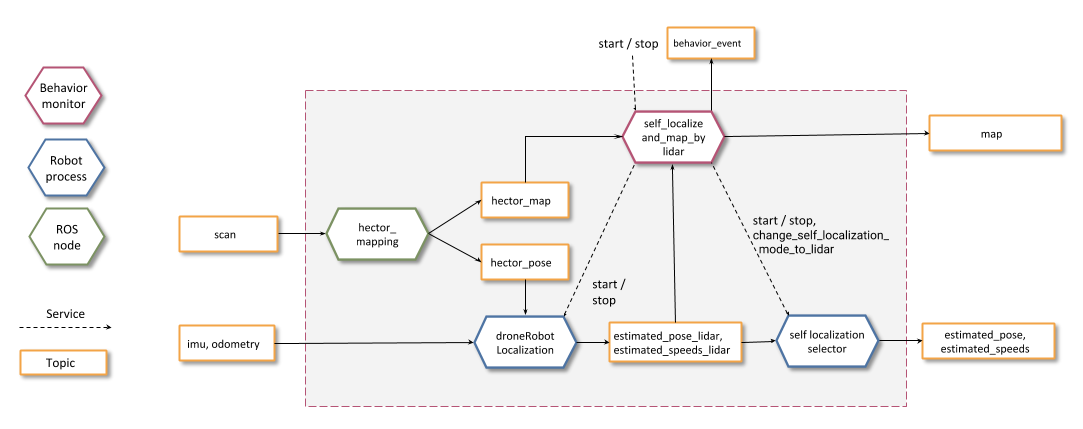
\includegraphics[width=\textwidth]{./Figures/BehaviorSlamArquitecture.png}
    \caption{Behavior self localize and map by lidar architecture. \textit{Hector mapping} is the SLAM module from \cite{hector_slam}. \textit{Drone Robot Localization} does the EKF. \textit{Self Localization Selector} gives the localization based on the selected technique.}
    \label{ch_4:fig:behav_slam}
  \end{figure}

  The estimated pose is then fed to the selector, which will toggle the localization technique. This implementation opens the door to new localization behaviors, a GPS based one for instance and also makes compatible the previous ones (visual markers based). It is easy to think of an scenario that requires both indoor and outdoor localization, in such a mission, the localization technique in use should be toggled in order for the navigator to work properly. As can be seen in Fig. \ref{ch_4:fig:behav_slam}, this is a \textit{Robot Process} with an added service to change the localization technique used.

  Bellow there is a list of the inputs and outputs of this behavior:

  % ToDo := Check this out with Martin
  [\textbf{ToDo := Set this up as a table??}]
  \begin{itemize}
  \item scan: This is the output of the lidar node, it is directly fed into the \textit{hector mapping} node
  \item imu: This topic contains the measures from the \textit{inertial measurement unit}
  \item odometry: This is a general topic with the measures from odometry
  \item map: This is the map as processed by the \textit{hector mapping} node
  \item estimated\_speed\_lidar: This is the estimated speed from the whole behavior process, fed to the selector
  \item estimated\_pose\_lidar: This is the estimated pose from the whole behavior process, fed to the selector
\end{itemize}

  This behavior monitors the correct working of the algorithm (\textit{hector mapping}) by listening on the \textit{map} topic, when it outputs strange or simply wrong data, an error is emitted.

  In the configuration file of this behavior the localization by visual markers behavior will appear as incompatible. As for the capabilities, all of \textit{hector mapping}, \textit{drone robot localization} and \textit{self localization selector} will figurate as capabilities, indicating that those processes should be started before this behavior.

\section{Navigation Interface} \label{ch_4:sect:nav_interface}

  We will consider the navigation interface as the minimum set of behaviors necessary to provide a robust, flexible API to do navigation tasks related to lidar-based localization and mapping techniques. It should be able to generate obstacle-free trajectories  to any given point (when there exists one) and be able to move the robot along those trajectories.

  The identified tasks for this API are as follows:

  \begin{enumerate}
    \item Given a point (or goal), execute the necessary motions to get the robot to that goal.
    \item Given a path, execute the necessary motions to follow it until the path is finished.
    \item Given a point (or goal), generate an obstacle-free path from the current robot's position to that goal.
  \end{enumerate}

  This tasks can be directly mapped with processes. However, we will implement them as separate behaviors to provide more modularity and reusability. Also, as each process will provide abstraction at a certain level of granularity, it makes sense to implement it as separate, independent behaviors (although some code will be duplicated)

  As of the current version of Aerostack, there exists a behavior that executes the motion of going to a given point in the 2D map representation used by Aerostack. However, this behavior is not general enough to be used with a different map representation, so we will implement a new one capable of executing the motion in the new map format: occupancy grids (which is the format used in \textit{hector mapping}). Also, in a dynamic environment, obstacles can arise in the path, this behavior will ensure that no collisions happen when executing the motion. More details to follow in section \ref{ch_4:subsect:behav_gtp}.

  The task of following a path or trajectory consists in instructing the previously available trajectory controller to follow a set of points (that conform the trajectory), given in a specific reference frame (world coordinates in this case). Contrary to the previously defined behavior, this one executes the motion blindly, providing a lower level of control to the user.

  For the last functionality, generating obstacle-free paths, another behavior will be implemented. It will consist mainly in a wrapper around the new planner, providing the lowest level of control in our navigation interface. For the planning we will employ a special planner provided as a ros package called \textit{move base}, which is specially crafted for lidar interfaces. It accepts an occupancy grid map and the raytraces from the lidar and implements the planning algorithm. Under the hood, it uses the elastic band algorithm for path optimization.

  The proposed names for each behavior are: \textit{behavior go to point in occupancy grid}, \textit{behavior follow path in occupancy grid}, \textit{behavior generate path in occupancy grid}. Figures \cref{ch_4:fig:behav_gtp,ch_4:fig:behav_fp,ch_4:fig:behav_gp} ilustrate the architecture followed by each of these behaviors. The following subsubsections explain each behavior in detail.

\subsection{Behavior Go to Point in Occupancy Grid} \label{ch_4:subsect:behav_gtp}

  This behavior provides the highest abstraction level of all the navigation interface, provided a target point, it will generate an obstacle-free trajectory to follow and send it to the trajectory controller, which executes the necessary motions to follow that trajectory. During the motion, this behavior will also ensure that no dynamic object gets in the way, recalculating the trajectory if necessary. In order to plan the trajectories, the new move base planner will be used, and as it will be a goal based behavior, the taget goal will be given as an argument to the start service. Figure \ref{ch_4:fig:behav_gtp} illustrates the general architecture of this behavior.

  \begin{figure}
    \centering
    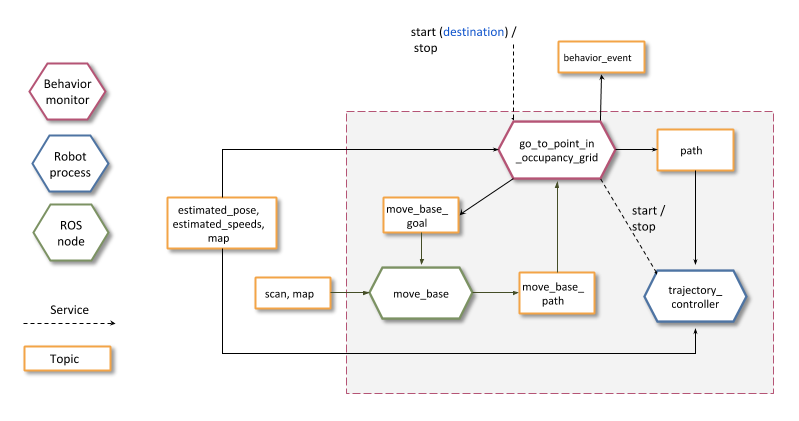
\includegraphics[width=\textwidth]{./Figures/BehaviorGTPArquitecture.png}
    \caption{Behavior Go to Point architecture. Move base is the planner}
    \label{ch_4:fig:behav_gtp}
  \end{figure}

  A condition for this behavior to operate correctly is that no other behavior is instructing the trajectory controller. To ensure this condition is met, the list of motion behaviors is stated as incompatible. The capabilities should list that it is a set-point-based flight behavior, instructing the behavior coordinator to setup the trajectory controller accordingly, the new planner (move base) should be explicitly declared as well so it is started automatically.

  \textbf{ToDo := Timeout if path not found?}

  The proposed topics will be:

  \textbf{ToDo := Set this up as a table}

  \begin{itemize}
    \item scan: Scan data from the lidar, direct input to the planner.
    \item map: Occupancy grid map from the self localize and map by lidar behavior, direct input to the planner.
    \item move base goal: Topic to instruct the planner to calculate an obstacle-free trajectory.
    \item move base path: Topic with the planned trajectory from the planner. Grabbed in the behavior to follow it.
  \end{itemize}


\subsection{Behavior Follow Path in Occupancy Grid}

  This behavior will communicate with the trajectory controller, instructing it to move following a given path received in the start service. For this behavior to work correctly, the motion behaviors should be disabled too. In this case, no other low level process is needed. The following figure illustrates the general concept (\ref{ch_4:fig:behav_fp}). Following a path can be a useful feature when developing fine grain controlled missions, like the ones enabled with Python.

  \begin{figure}[h]
    \centering
    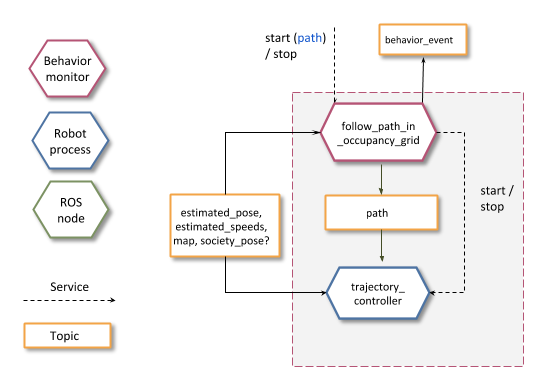
\includegraphics[width=0.75\textwidth]{./Figures/BehaviorFPArquitecture.png}
    \caption{Behavior follow path in occupancy grid architecture}
    \label{ch_4:fig:behav_fp}
  \end{figure}

  Again, the correct settings should be ensured in the configuration file, marking motion behaviors to avoid trajectories interferences.

\subsection{Behavior Generate Path in Occupancy Grid}

  In this case we will only implement a wrapper around the move base planner. This is the lowest abstraction level provided by the navigation interface API. Being able to generate paths can be useful for fine grain controlled missions and debugging. The only communication way for this behavior will be dropping the planned the path on the belief memmory, this way the amount of traffic and topics is reduced, saving computing resources and avoiding polluting more topics. It's architecture is depicted in figure \ref{ch_4:fig:behav_gp}.

  \pagebreak

  \begin{figure}[h]
    \centering
    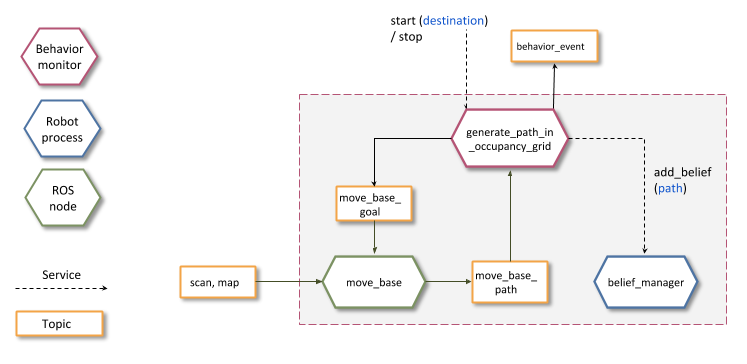
\includegraphics[width=0.85\textwidth]{./Figures/BehaviorGPArquitecture.png}
    \caption{Behavior generate path in occupancy grid architecture}
    \label{ch_4:fig:behav_gp}
  \end{figure}


This chapter has reviewed the most important aspects and specification of the implemented modules. In the next one, the validation and testing for these behaviors will be introduced.

\begin{comment}
  \begin{itemize}
  \end{itemize}
\end{comment}
 % Experimental Setup
  \chapter{Validation} \label{ch_5:chapter}

  This chapter will go through all the validation and tests implemented to measure the performance and the correct functioning of the new behaviors. 

  To validate each implemented behavior we propose using them both in simulation and in real flight missions. The validation tests are presented in detail in section \ref{ch_5:sect:val_tests}, explaining what the tests measure and how they do it as well as the intuition behind each test. Afterwards, in section \ref{ch_5:sect:experiments} we explain in detail the mission implemented for each behavior along with further information of the simulator employed in section \ref{ch_5:subsect:exp_simulation}. The simulation integration with the current version of Aerostack and the specific details of the real flight aircraft are detailed in section \ref{ch_5:subsect:exp_real_flight}. Section \ref{ch_5:sect:results} reports on the results obtained for each mission both in sumulation and in real flight and \ref{ch_5:sect:discussion} closes the chapter with the discussion of the results.
 
\section{Validation Tests} \label{ch_5:sect:val_tests}

  A validation test should ensure that the behavior complies with the following constraints:

  \begin{enumerate}
    \item \underline{Functioning}: It should do what it is supposed to do. No more, no less.
    \item \underline{Requirements}: It should meet the imposed requirements (explained in \ref{ch_4:sect:requirements})
  \end{enumerate}

  The first constraint is the most obvious, a behavior is designed to do a concrete task. It should do only what is designed to do. The idea behind a behavior is to encapsulate a concrete algorithm, it can be the layer that encapsulates the algorithm, providing a standard API access, but it can only be one functionality.

  To test this constraint we will provide both a simulation and a real mission and put to work each behavior independently, testing that each one works as expected. We will measure the precision of each behavior based on the amount of the task that it is able to complete without errors.

  One of the hardest requirements to meet is that of the performance, any implemented behavior should be efficient enough to run both onboard and in ground control stations in real time. Although this requirement could not be a problem for a PC it surely can be a problem on onborad computers. Also, it is difficult to measure as it is not possible to isolate the behaviors from the Aerostack platform. A possibility could be to run the Aerostack without the behaviors, in idle and measure and then add the behaviors and measure again. In any case, measuring the performance in idle is not very representative in this case. Instead, what we will do is put the system to work and test whether it crashes or drops frames.

\section{Simulation} \label{ch_5:sect:simulation}

  The chosen simulator for these tests is Gazebo Sim (\cite{gazebo_web}), an open source, multiplatform, robot simulator. It was chosen because of it's open source nature, ease of use and great integration with ROS. Gazebo features an open, modular, plugin based architecture, which makes it perfect to integrate new components and opens the door for modules being simulated inside it and the outside world. In our case, to communicate the simulated UAV with ROS and the Aerostack framework.

  In order to convey the simulator with ROS we will employ an already made plugin called RotorS \cite{rotors2016}. RotorS provides some UAV models and a plugin that translates gazebo topics to ROS ones, unifying the access to the data. This architecture is perfect for any robotic environment as it minimizes the overhead of changing from simulation to real flight, as long as the topics are called the same, the Aerostack framework does not even notice it.

  As all the simulation is launched with configuration files and was done with flexibility in mind, we could adapt the already available configurations to our needs, minimizing the overhead of naming topics to our conventions.

  To choose a UAV model from the available ones we looked up for one that matches our requirements, namely a lidar sensor (hokuyo if possible), a front camera and an altitude sensor. RotorS provides a UAV modeled after the AscTec Hummingbird \cite{hummingbird_web} drone, which meets all these requirements.

\section{Real Flight} \label{ch_5:sect:real_flight}

  Our requirements came mainly because of the implemented behaviors, which in turn came from the available hardware in the research group. Currently, the aircraft used for the most important missions is a Matrice 100 from DJI (\cite{dji_matrice_web}) with all the sensorization cited above.

  This is used because of it's extendability (any sensor platform can be plugged in), open API and powerful motors. It's verstaile enough to provide a testbed for many research experiments and the battery lasts enough for medium duration missions.

\section{Testing Mission} \label{ch_5:sect:testing_mission}

  To provide the most realistic environment possible, the mission used to conduct all the experiments will be based in a real assignment requested to the research group a few months ago. The mission consists in inspecting the internal facade of a plant's boiler. At the time of request this new navigation interface was not implemented, so the flight was made almost by hand. In fact, this inteface was proposed after the need of an autonomous flight navigator whith the available hardware.

  The idea behind the mission is to fly a drone along the facade filming all the breathers, after the mission is completed, the film is extracted and given to the plant experts for their analysis. Additionally, a handmade mission could be very costly for the gas company as they would have had to install a portable crane and put a human to do the inspection of the 40 meters long facade.

  A human commanded drone accomplished the whole inspection in less than one hour. Furthermore, even in that case it was challenging for the human operator as he had to fly near the wall, which causes the drone to destabilize due to the air flows. This is the point where autonomous navigation comes in. In an autonomous mission, the control loop can be closed with any parameter that can be measured, in this case, the go to point behavior could have been employed to make the aircraft fly upwards until the whole boiler is inspected and then commanded back to land at a certain point.

  As the job is already done it is not possible to replicate it, hence we propose to simulate a boiler in Gazebo that resembles to the real mission and the inspection of an internal facade in a building for the real flight.

  The next sections will deepen in all the details of the conduted experiments and the results obtained during the tests.

\section{Experiments} \label{ch_5:sect:experiments}

  As mentioned before, for each behavior we will ensure it complies with our constraints: correct functioning and requirements (performance mostly).
  
  Once the whole Aerostack system is deployed, the first test for each behavior consists in checking it's activation conditions, i.e.: the \textit{behavior self localize and map by lidar} cannot work without a lidar, deploying the whole Aerostack in a lidar-less UAV should cause the behavior to be deactivated instantly.

  This way we tested all conditions and capabilities of all the proposed behaviors. As this is all software related, we easily corrected all the bugs found. One example of this was the access to the path planner module: The new planner (\textit{move base}) can only plan to one goal, this makes all the behaviors requiring this module mutually incompatible, namely, the behavior that generates paths cannot work simultaneously with that of the go to point . In the same fashion the behaviors that make use of the trajectory planner cannot work together or a collision could occur.

  For the functioning constraint we setup both the real and simulated missions with a python script that commands the Aerostack, if after doing a certain amount of missions, the behaviors work as expected we consider that they work correctly. 
  
  The following subsections explain the implemented mission for each behavior. Note that, the first two missions where only tested on the simulated environment to minimize the human operator time needed for the tests. For all missions both the simulation and the real environments used are the same, nothing was changed in the environment.

  \subsection{Behavior Generate Path in Occupancy Grid} \label{ch_5:subsect:behav_genpath_mission}

    This mission was only tested in simulation, it consisted in generating a path for every point in the go to point mission (sect. \ref{ch_5:subsect:behav_gtp_mission}). After the mission is finished, $6$ paths should be present in the belief memory. Therefore the mission can be described as follows:
    
    \begin{enumerate}
      \item Generate path for point: [0, 0, 1.5]
      \item Generate path for point: [1, 0, 1.5]
      \item Generate path for point: [1, 0, 10]
      \item Generate path for point: [1, -5, 10]
      \item Generate path for point: [0, -5, 1.5]
      \item Generate path for point: [0, -5, 1]
    \end{enumerate}

    The full python source code can be found in the appendix \ref{app1:generate_path_mission}

  \subsection{Behavior Follow Path in Occupancy Grid} \label{ch_5:subsect:behav_fpath_mission}

  In this mission we employ the previous behavior to generate paths from the current position to the target point and fed it as input parameter to this behavior. Working in tandem, these behaviors do a similar job to the go to point one (without the obstacle avoidance). The generated mission is outlined as:

    \begin{enumerate}
      \item Follow path for point: [0, 0, 1.5]
      \item Follow path for point: [1, 0, 1.5]
      \item Follow path for point: [1, 0, 10]
      \item Follow path for point: [1, -5, 10]
      \item Follow path for point: [0, -5, 1.5]
      \item Follow path for point: [0, -5, 1]
    \end{enumerate}

    The python code for this mission can be found in the appendix \ref{app1:follow_path_mission}

  \subsection{Behavior Go To Point in Occupancy Grid} \label{ch_5:subsect:behav_gtp_mission}

    This is the centre key of the navigation system, providing the most rich, autonomous behavior. The mission is as simplified version of the one made for the real boiler inspection, but fitted to the real flight scenario at hand. It's outline is presented below:

    \begin{enumerate}
      \item Take Off
      \item Go to $1.5$ meters height ([0, 0, 1.5])
      \item Go to $1$ meter to the front, maintaining the altitude. ([1, 0, 1.5])
      \item Go to $10$ meters height, maintaining the same distance to the wall. ([1, 0, 10])
      \item Go to $5$ meters to the right, keeping the same distance and altitude. ([1, -5, 10])
      \item Go to $1$ meter away from the wall, maintaining the same altitude. ([0, -5, 1.5])
      \item Go to $1$ meter height, maintaining the same distance to the wall. ([0, -5, 1])
      \item Land
    \end{enumerate}

    Please, find all the python code for this mission attached in the appendix \ref{app1:go_to_point_mission}.

  \subsection{Simulation} \label{ch_5:subsect:exp_simulation}

    \begin{figure}[!h]
      \centering
      \includegraphics[width=0.9\textwidth,height=0.4\textheight,keepaspectratio]{./Figures/BoilerSim.png}
      \caption{Simulated boiler. $57$ meters tall by $16$ meters (square section). The UAV is enclosed in the yellow circle.}
      \label{ch_5:fig:boiler_sim}
    \end{figure}

    For the simulation we created a blender model of a boiler and exported it to Gazebo, then we created a RotorS enabled Gazebo world with the hummingbird drone model. The dimensions of the simulated boiler are listed in table \ref{ch_5:table:boiler_sim_dims}. To get an idea of the proportions of the boiler with the aircraft see figure \ref{ch_5:fig:boiler_sim}. The drone has been outlined in yellow, it almost unseeable.

    \begin{table}[!h]
      \centering
      \begin{tabular}{lr} \toprule
        \multicolumn{2}{c}{\textit{Simulated boiler dimensions}}        \\ \midrule
        Width $\times$ Depth $\times$ Height & $16 \times 16 \times 57$ \\ \bottomrule
        \hline
      \end{tabular}
      \caption{Simulation computer specifications}
      \label{ch_5:table:boiler_sim_dims}
    \end{table}

    The specifications of the computer employed for all the simulations are depicted in the following table \ref{ch_5:table:laptop_specs}:

    \begin{table}[!h]
      \centering
      \begin{tabular}{lr} \toprule
        \multicolumn{1}{c}{\textit{component}} & \multicolumn{1}{c}{\textit{value}}   \\ \midrule
        Ram           & DDR 4 32 GB     \\
        Processor     & 3.4 Ghz 8 cores \\
        GPU           & GTX 1050 Ti     \\ \bottomrule
        \hline
      \end{tabular}
      \caption{Simulation computer specifications}
      \label{ch_5:table:laptop_specs}
    \end{table}

    In this scenario, performance does not comprise a problem because with enough GPU, the simulation can run smoothly and all processes can run with good memory support.

    Figure \ref{ch_5:fig:full_sim} shows the simulated world running inside gazebo, along with the camera output and a visualization of the current lidar map.
    
    \begin{figure}
      \centering
      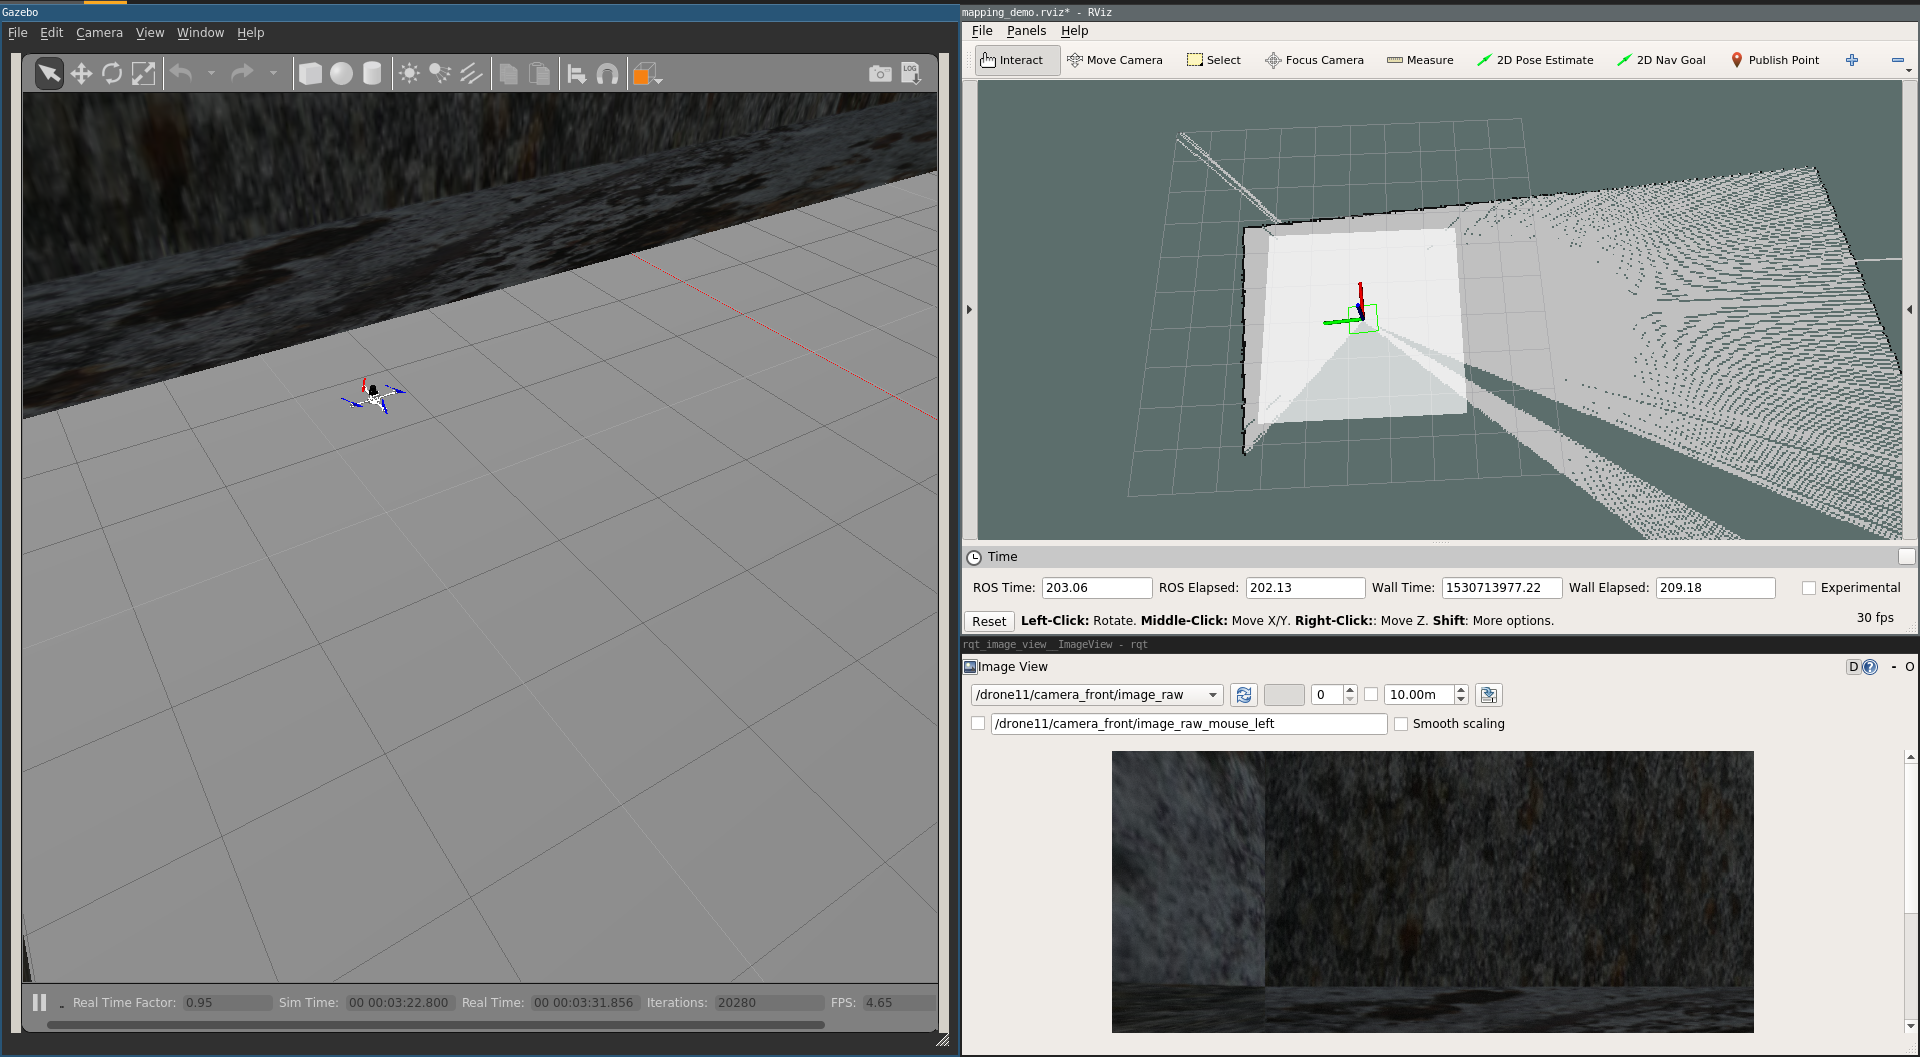
\includegraphics[width=0.9\textwidth,height=0.5\textheight,keepaspectratio]{./Figures/FullSim.png}
      \caption{Gazebo and Rviz. Simulation visualization during the execution of the mission. Left: Gazebo World, top-right: Rviz lidar measures, bottom-right: Hummingbird front camera}
      \label{ch_5:fig:full_sim}
    \end{figure}

  \subsection{Real Flight} \label{ch_5:subsect:exp_real_flight}

    For the real flight tests we used the sports centre in the School of Industrial Engineers, which is a closed space that can serve for our purposes, it's dimensions are listed in table \ref{ch_5:table:sports_dims}.

    \begin{table}[!h]
      \centering
      \begin{tabular}{lr} \toprule
        \multicolumn{2}{c}{\textit{Sports Centre Dimensions}}        \\ \midrule
        Width $\times$ Depth $\times$ Height & $10 \times 25 \times 14$ \\ \bottomrule
        \hline
      \end{tabular}
      \caption{Dimensions of the sports centre used for real flight tests. School of Industrial Engineers}
      \label{ch_5:table:sports_dims}
    \end{table}

    \begin{figure}
      \centering
      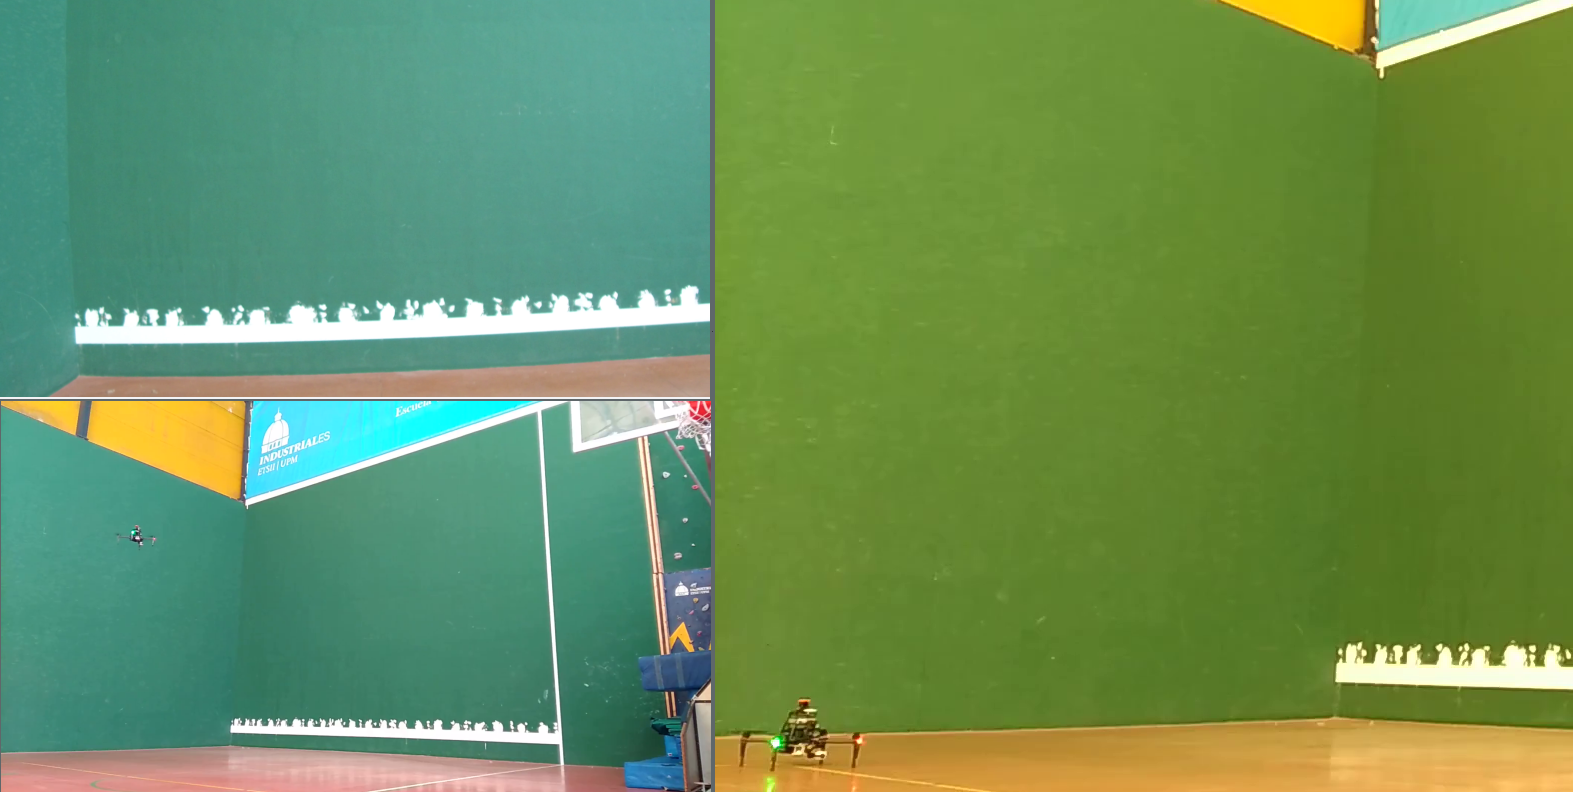
\includegraphics[width=0.9\textwidth,height=0.5\textheight,keepaspectratio]{./Figures/RealFlight.png}
      \caption{DJI Matrice 100 drone in the real flight mission, School of Industrial Engineers Sports centre. Top left: Front camera from the drone before the mission. Bottom left: drone flying during the mission. Right: closeup of the landed drone before the mission.}
      \label{ch_5:fig:full_realflight}
    \end{figure}


    The chosen drone ships a DJI Manifold micro computer for onboard computation (\cite{dji_manifold_web}). Its technical details are contained in table \ref{ch_5:table:manifold_specs}

    \begin{table}[!h]
      \centering
      \begin{tabular}{lr} \toprule
        \multicolumn{1}{c}{\textit{component}} & \multicolumn{1}{c}{\textit{value}}   \\ \midrule
        Ram           & DDR 3 2 GB     \\
        Processor     & 2.5 Ghz 4 cores \\
        GPU           & NVIDIA Kepler GeForce \\ \bottomrule
        \hline
      \end{tabular}
      \caption{Onboard computer specification}
      \label{ch_5:table:manifold_specs}
    \end{table}

    Onboard computation is the better option in this case because there is no \textit{auto pilot} (fallback driver controller, shipped in many commercial drones to do automatic hover when no orders are received) and given the distances it can travel and the altitude, ensuring WiFi coverage is difficult. Hence, the most secure option is to load all the necessary software inside the onboard computer and send just a few orders from the ground control station. More specifically, launch the Aerostack and the python mission.

    The manifold computer is not very powerful so special attention must be put on performance , if computing power drains it can be catastrophic. To aid in this situation a human pilot was prepared to take control during all the tests, although at the end it was not necessary.

\section{Experimental Results} \label{ch_5:sect:results}

  This section will explain the results obtained, we will first go through the simulation results and continue with the real flight ones. For each behavior, \cref{ch_5:table:generate_path_results,ch_5:table:follow_path_results,ch_5:table:go_to_point_results,ch_5:table:real_flight_results} show: the correct execution of the behavior, the mean and standard deviation execution time for all points and the total time of the mission, also, the last row shows the averaged scores and times. Everything is measured in minutes and each experiment is run ten times, also, the timeout counter for each behavior is set to 4 minutes.
 
  \begin{table}[!h]
  \centering
  \begin{tabular}{lccr} \toprule
    \multicolumn{4}{c}{\textit{Generate Path in Occupancy Grid}}                        \\ \midrule
    \textit{Test Number} & \textit{Correct} & \textit{Point time} & \textit{Total time} \\ \midrule
      1 & 6/6 & 0.21 ($\pm$ 0.01) & 1.25 \\ \hline
      2 & 6/6 & 0.20 ($\pm$ 0.00) & 1.20 \\ \hline
      3 & 6/6 & 0.20 ($\pm$ 0.00) & 1.20 \\ \hline
      4 & 6/6 & 0.20 ($\pm$ 0.00) & 1.20 \\ \hline
      5 & 6/6 & 0.20 ($\pm$ 0.00) & 1.20 \\ \hline
      6 & 6/6 & 0.20 ($\pm$ 0.00) & 1.20 \\ \hline
      7 & 6/6 & 0.20 ($\pm$ 0.00) & 1.20 \\ \hline
      8 & 6/6 & 0.20 ($\pm$ 0.00) & 1.20 \\ \hline
      9 & 6/6 & 0.20 ($\pm$ 0.00) & 1.20 \\ \hline
      10 & 6/6 & 0.20 ($\pm$ 0.00) & 1.20 \\ \hline
      \textit{\#} & \textit{Total Correct} & \textit{Avg. Total Point time} & \textit{Avg. Total time} \\ \midrule
      - & 60/60 (100\%) & 0.20 ($\pm$ 0.00) & 1.20 ($\pm$ 0.01) \\ \bottomrule
      \hline
  \end{tabular}
  \caption{Results from \textit{generate path} behavior, run accross 10 tests. Correct executions, averaged execution time for all 6 points and total execution of the mission. Measured in minutes}
  \label{ch_5:table:generate_path_results}
\end{table}


  Table \ref{ch_5:table:generate_path_results} shows the results for the behavior \textit{generate path in occupancy grid}. Since this behavior does not perform any motion, it is just planning, a $100\%$ hits seems reasonable, it means that the planner does its job correctly, both the move base planner and the path planner modules work correctly, also, the behavior works as expected, generating all the requested paths and inserting them in the belief memory. Furthermore, the times employed to generate the trajectories are very stable, which meets our requirements. 

  \begin{table}[!h]
  \centering
  \begin{tabular}{lccr} \toprule
    \multicolumn{4}{c}{\textit{Follow Path in Occupancy Grid}}                        \\ \midrule
    \textit{Test Number} & \textit{Correct} & \textit{Point time} & \textit{Total time} \\ \midrule
      1 & 5/6 & 1.68 ($\pm$ 1.60) & 10.75 \\ \hline
      2 & 2/6 & 2.70 ($\pm$ 1.84) & 16.91 \\ \hline
      3 & 4/6 & 1.85 ($\pm$ 1.65) & 11.70 \\ \hline
      4 & 3/6 & 2.24 ($\pm$ 1.57) & 13.96 \\ \hline
      5 & 3/6 & 2.61 ($\pm$ 1.65) & 16.24 \\ \hline
      6 & 4/6 & 1.86 ($\pm$ 1.64) & 5.75 \\ \hline
      7 & 6/6 & 0.87 ($\pm$ 0.77) & 9.95 \\ \hline
      8 & 6/6 & 1.02 ($\pm$ 0.89) & 6.61 \\ \hline
      9 & 4/6 & 2.38 ($\pm$ 1.67) & 14.77 \\ \hline
      10 & 5/6 & 1.62 ($\pm$ 1.34) & 10.33 \\ \hline
      \textit{-} & \textit{Total Correct} & \textit{Avg. Total Point time} & \textit{Avg. Total time} \\ \midrule
      - & 42/60 (0.70) & 1.88 ($\pm$ 0.59) & 11.70 ($\pm$ 3.60) \\ \bottomrule
      \hline
  \end{tabular}
  \caption{Results from \textit{Follow Path} behavior, run accross 10 tests. Correct executions, averaged execution time for all 6 points and total execution of the mission. Measured in minutes}
  \label{ch_5:table:go_to_point_results}
\end{table}


  The follow path in occupancy grid behavior had the worst performance of all, although it scores for 65\% of the points, it has a lot of variability, this may be due to the fact that it executes the motions blindly, no logic is applied to recalculate paths when needed, it just executes the given trajectory. This behavior is slighty more complicated than the previous one in the sense that it has to execute motions, which increases the difficulty.

  We acknowledged various fault causes, the very first one is estimation, although some points where not perfectly matched, the end positions where very close to the goal. This drift in localization arises from the lack of fine tuning, the localization EKF is not completely tuned for simulatation of the UAV. Also, during the tests we observed that the trajectory controller has some weird behaviors. There were various cases where the orders took no effect. As of the time of writing, the controller is being remade from the ground up.

  Not matching the target points means that the behavior does not finish and it only stops when the timeout is reached. This faulty finish condition, in turn adds up to the execution time, which explains some of the large times of execution. Tests 2, 4, 5 and 9 accounts for this fact, they score the least and also last the most. Interestingly enough, this test has more fully completed missions that the one of \textit{go to point}, 2 out of 10 versus 1 out time, but in general has more faulty points, rising the global time of execution for the whole test.

  \begin{table}[!h]
  \centering
  \begin{tabular}{lccr} \toprule
    \multicolumn{4}{c}{\textit{Go to Point in Occupancy Grid}}                        \\ \midrule
    \textit{Test Number} & \textit{Correct} & \textit{Point time} & \textit{Total time} \\ \midrule
      1 & 4/6 & 1.78 ($\pm$ 1.74) & 11.21 \\ \hline
      2 & 3/6 & 2.42 ($\pm$ 1.64) & 15.07 \\ \hline
      3 & 3/6 & 2.43 ($\pm$ 1.66) & 15.13 \\ \hline
      4 & 4/6 & 1.72 ($\pm$ 1.69) & 10.85 \\ \hline
      5 & 3/6 & 2.40 ($\pm$ 1.66) & 14.91 \\ \hline
      6 & 5/6 & 1.36 ($\pm$ 1.29) & 8.68 \\ \hline
      7 & 4/6 & 1.71 ($\pm$ 1.69) & 10.77 \\ \hline
      8 & 5/6 & 1.37 ($\pm$ 1.33) & 8.75 \\ \hline
      9 & 6/6 & 0.79 ($\pm$ 0.77) & 5.28 \\ \hline
      10 & 4/6 & 2.19 ($\pm$ 1.57) & 13.68 \\ \hline
      \textit{-} & \textit{Total Correct} & \textit{Avg. Total Point time} & \textit{Avg. Total time} \\ \midrule
      - & 41/60 (0.68) & 1.82 ($\pm$ 0.52) & 11.43 ($\pm$ 3.12) \\ \bottomrule
      \hline
  \end{tabular}
  \caption{Results from \textit{Go to Point} behavior, run accross 10 tests. Correct executions, averaged execution time for all 6 points and total execution of the mission. Measured in minutes}
  \label{ch_5:table:go_to_point_results}
\end{table}


  The go to point behavior is most complex, but also more stable than the previous one, it contains some logic to handle obstacles and track the drone position. Nevertheless, the bad matching of points is a problem, this is the case of the 2nd, 3rd and 5th tests, which fail to reach half of the points, rising the execution time to 15 minutes at worst, the correlation is clear. We strengthen our assumption with tests 8th and 9th, that amounts for 5 out of 6 and 6 out 6 goals reached, respectively, with the lowest times of all the tests. The implemented behavior works correctly in 68\% of the cases, which is not bad given the complexity in coordination needed to accomplish the task and the short time employed implementing it.

  The last test in our experiments are run in real flight, with the previously explained drone and environment. Due to time constraints and both hardware and pilot availability, we ran only 3 tests, the results are reported in table \ref{ch_5:table:real_flight_results}

  \begin{table}[!h]
  \centering
  \begin{tabular}{lccr} \toprule
    \multicolumn{4}{c}{\textit{Real Flight - Go to Point behavior}}                        \\ \midrule
    \textit{Test Number} & \textit{Correct} & \textit{Point time} & \textit{Total time} \\ \midrule
      1 & 4/6 & 1.26 ($\pm$ 0.92) & 7.91 \\ \hline
      2 & 6/6 & 0.71 ($\pm$ 0.37) & 4.78 \\ \hline
      3 & 6/6 & 0.84 ($\pm$ 0.31) & 5.24 \\ \hline
      \textit{\#} & \textit{Total Correct} & \textit{Avg. Total Point time} & \textit{Avg. Total time} \\ \midrule
      - & 16/18 (0.88\%) & 0.94 ($\pm$ 0.23) & 5.97 ($\pm$ 1.38) \\ \bottomrule
      \hline
  \end{tabular}
  \caption{Results from \textit{Go to Point} behavior in real flight, run accross 3 tests. Correct executions, averaged execution time for all 6 points and total execution of the mission. Measured in minutes}
  \label{ch_5:table:real_flight_results}
\end{table}


  It is worth noting that these tests are much more robust and fast, the intuition behind these results is that the localization module is widely tested and tuned for this specific aircraft which makes sense given that it is used for industrial level real flight missions. Also, the speed of this drone is comparably higher.

  Although these tests were run with a human operator fallback, just in case something went wrong, none of the tests required it. Even in the first test, where two points failed to match, the system recovered and successfully finished the mission. Furthermore, the two failed points where encountered when reaching the highest altitude and when moving away from the wall at highest altitude, points 4 and 6, respectively (refer to \ref{ch_5:subsect:behav_gtp_mission} for detailed coordinates). Our best guess for this performance is based on the environment: the sports centre walls are made of various materials, it has about 8-9 meters of solid wall and then a grid gate with holes to the roof. We believe that the holes in the grid gate tricked the lidar based localization, which in turn caused the go to point not to match the target point. Also, as the localization is made out of the fusion of various sensor inputs, this phenomenon does not happen always, which is another proof of the robustness of the system.

  \subsection{Performance}

  As stated before, measuring the performance was difficult, but we took some notes. We acknowledged that the planning system delayed the whole system, dropping some frames from the \textit{scan} topic. We believe this is related to the duplication of the \textit{map} topic in the \textit{self localize and map behavior}, our intuition behind this is the fact that map is a topic that transports dense data at a high ratio, hence this could be a problem in the future, when more intensive modules are added.

  In any case, we did not recognize any significant problem in the execution of any of the tests. Even the real flight mission ran smoothly and without problems.

\section{Discussion} \label{ch_5:sect:discussion}

  The results obtained shed some light over the problems that arise in an autonomous navigation system, clarifying the need for more tests and a better prepared simulation environment. Also, the implemented behaviors could work better with a more robust trajectory controller and more warranties from the planner, this could help to isolate the behaviors functioning from the rest of the stack they depend upon, unmasking possible errors and helping to debug them.

  Also, the environment used for simulation is very well suited for our needs, but lacks some tuning. The fact that there exists such difference between  the real flight mission and the simulated one is not good, although clearly improvable through extensing tuning and testing. Even though, the proposed system works reasonably well for the time invested in implementation and also highlights that we are on the correct track for future experiments.

This chapter presented all the validation missions and environment employed for testing all the implemented behaviors, also the results were presented and analyzed for discussion. The next chapter will conclude the thesis adding more in depth thoughts about the results obtained and further research.
 % Validation of the experiments
  \chapter{Conclusions \& Further Research}

This chapter will conclude the thesis with our conclusions on the conducted experiments and the proposed system and expose the open lines of study we would like to target our research to. 

\section{Conclusions} \label{ch_6:sect:conclusions}

  At the sight of the results obtained it is clear for us that we are on the right track towards a fully autonomous navigation system. We would like to stress out that, as far as the navigation system is supported by an aerial architecture, it depends upon its correct functioning. In fact, in our experiments, the biggest source of failure was the slam module, although the employed technique is very advanced and stands over the state of the art papers, it fails in some situations, propagating the error above until higher levels of abstraction: the Behavioral system, where we implemented the whole navigation system.

  In this thesis we delved into different high level abstractions for the construction of a fully autonomous navigation system, we proposed a system based on the most up to date theory in planning and localization, we prepared some experiments to test our research hypotheses and implemented all the behaviors it is composed of. Also, we counted on the necessary resources both in hardware and in time to conduct all the tests, and at the end, we proved that the Aerostack system is the perfect testbed for artificial intelligence algorithms aimed at aerial robotics.

\pagebreak

\section{Further Research} \label{ch_6:sect:research}

  It is only through extensive and stressful tests that a system like this can prove useful and bullet proof. In the future, we would like explore the robustness and reliability of the proposed system under the conditions of more difficult environments, as well as to test it on a real life, business oriented mission, which is where the inspiration for this whole work.

  After all the tests conducted, it is clear that the localization subsystem is the key to more reliable, successful intelligent behaviors, is the basement for higher levels of abstraction. We would like to strengthen these lower level algorithms first in order to improve the base system and open the door for more intelligent, autonomous behaviors, maybe in the future more complex missions can be achieved with this system based solely on a few sources of data.
 % Conclusions and future reseach
  \backmatter
%% ----------------------------------------------------------------
%% ----- Bibliography ---------------------------------------------
  \label{Bibliography}
  \lhead{\emph{Bibliography}}  % Change the left side page header to "Bibliography"
  \printbibliography
  % \bibliographystyle{unsrtnat}  % Use the "unsrtnat" BibTeX style for formatting the Bibliography
  % \bibliography{Bibliography}  % The references (bibliography) information are stored in the file named "Bibliography.bib"
%% ----------------------------------------------------------------
%% ----- Appendices -----------------------------------------------
  % Now begin the Appendices, including them as separate files

  \mainmatter
  \addtocontents{toc}{\vspace{2em}} % Add a gap in the Contents, for aesthetics

  \appendix % Cue to tell LaTeX that the following 'chapters' are Appendices

  \lhead{\emph{Appendix}}  % Change the left side page header to "Bibliography"

  \chapter{An Appendix}

Lorem ipsum dolor sit amet, consectetur adipiscing elit. Vivamus at pulvinar nisi. Phasellus hendrerit, diam placerat interdum iaculis, mauris justo cursus risus, in viverra purus eros at ligula. Ut metus justo, consequat a tristique posuere, laoreet nec nibh. Etiam et scelerisque mauris. Phasellus vel massa magna. Ut non neque id tortor pharetra bibendum vitae sit amet nisi. Duis nec quam quam, sed euismod justo. Pellentesque eu tellus vitae ante tempus malesuada. Nunc accumsan, quam in congue consequat, lectus lectus dapibus erat, id aliquet urna neque at massa. Nulla facilisi. Morbi ullamcorper eleifend posuere. Donec libero leo, faucibus nec bibendum at, mattis et urna. Proin consectetur, nunc ut imperdiet lobortis, magna neque tincidunt lectus, id iaculis nisi justo id nibh. Pellentesque vel sem in erat vulputate faucibus molestie ut lorem.

Quisque tristique urna in lorem laoreet at laoreet quam congue. Donec dolor turpis, blandit non imperdiet aliquet, blandit et felis. In lorem nisi, pretium sit amet vestibulum sed, tempus et sem. Proin non ante turpis. Nulla imperdiet fringilla convallis. Vivamus vel bibendum nisl. Pellentesque justo lectus, molestie vel luctus sed, lobortis in libero. Nulla facilisi. Aliquam erat volutpat. Suspendisse vitae nunc nunc. Sed aliquet est suscipit sapien rhoncus non adipiscing nibh consequat. Aliquam metus urna, faucibus eu vulputate non, luctus eu justo.

Donec urna leo, vulputate vitae porta eu, vehicula blandit libero. Phasellus eget massa et leo condimentum mollis. Nullam molestie, justo at pellentesque vulputate, sapien velit ornare diam, nec gravida lacus augue non diam. Integer mattis lacus id libero ultrices sit amet mollis neque molestie. Integer ut leo eget mi volutpat congue. Vivamus sodales, turpis id venenatis placerat, tellus purus adipiscing magna, eu aliquam nibh dolor id nibh. Pellentesque habitant morbi tristique senectus et netus et malesuada fames ac turpis egestas. Sed cursus convallis quam nec vehicula. Sed vulputate neque eget odio fringilla ac sodales urna feugiat.

Phasellus nisi quam, volutpat non ullamcorper eget, congue fringilla leo. Cras et erat et nibh placerat commodo id ornare est. Nulla facilisi. Aenean pulvinar scelerisque eros eget interdum. Nunc pulvinar magna ut felis varius in hendrerit dolor accumsan. Nunc pellentesque magna quis magna bibendum non laoreet erat tincidunt. Nulla facilisi.

Duis eget massa sem, gravida interdum ipsum. Nulla nunc nisl, hendrerit sit amet commodo vel, varius id tellus. Lorem ipsum dolor sit amet, consectetur adipiscing elit. Nunc ac dolor est. Suspendisse ultrices tincidunt metus eget accumsan. Nullam facilisis, justo vitae convallis sollicitudin, eros augue malesuada metus, nec sagittis diam nibh ut sapien. Duis blandit lectus vitae lorem aliquam nec euismod nisi volutpat. Vestibulum ornare dictum tortor, at faucibus justo tempor non. Nulla facilisi. Cras non massa nunc, eget euismod purus. Nunc metus ipsum, euismod a consectetur vel, hendrerit nec nunc.  % Appendix Title
  %\input{Appendices/AppendixB} % Appendix Title
  %\input{Appendices/AppendixC} % Appendix Title

  \addtocontents{toc}{\vspace{2em}}  % Add a gap in the Contents, for aesthetics
  \backmatter
%% ----------------------------------------------------------------
\end{document}  % The End
